\section{Results}
\label{sec:results}

\subsection{SAE features dominate raw neurons on concept F1 (sanity reproduction)}
\label{ssec:res_f1}

We first verify that our pipeline reproduces the qualitative finding of \citet{simon2024interplm}: \sae features cover more biological concepts than raw \plm neurons at higher F1 thresholds. \Tabref{tab:f1_compare} reports the counts.

\begin{table}[h]
\centering
\caption{Number of units at increasing F1 thresholds. \sae features ($n{=}10{,}240$) versus raw \esm-8M layer-4 neurons ($n{=}320$) under the same threshold sweep. Best results in {\bf bold}.}
\label{tab:f1_compare}
\begin{tabular}{@{}lccc@{}}
\toprule
\textbf{Threshold} & \textbf{\sae features} & \textbf{\esm neurons} & \textbf{Ratio} \\
\midrule
Max-F1 $\geq 0.5$ & \textbf{165} & 29  & 5.7$\times$ \\
Max-F1 $\geq 0.4$ & \textbf{365} & 129 & 2.8$\times$ \\
Max-F1 $\geq 0.3$ & \textbf{771} & 298 & 2.6$\times$ \\
Max-F1 $\geq 0.2$ & \textbf{1{,}648} & 320 & 5.2$\times$ \\
\midrule
Best F1 (any unit) & \textbf{0.932} & 0.753 & 1.24$\times$ \\
Concepts at F1 $\geq 0.5$ & 5 / 15 & 4 / 15 & --- \\
\bottomrule
\end{tabular}
\end{table}

At F1 $\geq 0.5$ the \sae has 5.7$\times$ more aligned units than the dense neuron basis, matching the InterPLM headline ratio on a smaller corpus. The 165/29 absolute counts are lower than InterPLM's 2{,}548/46 because we evaluate on 1{,}500 proteins versus full \swissprot, with 16 concepts versus 433 and a coarser five-percentile sweep. The relative gap is intact.

\begin{figure}[h]
\centering
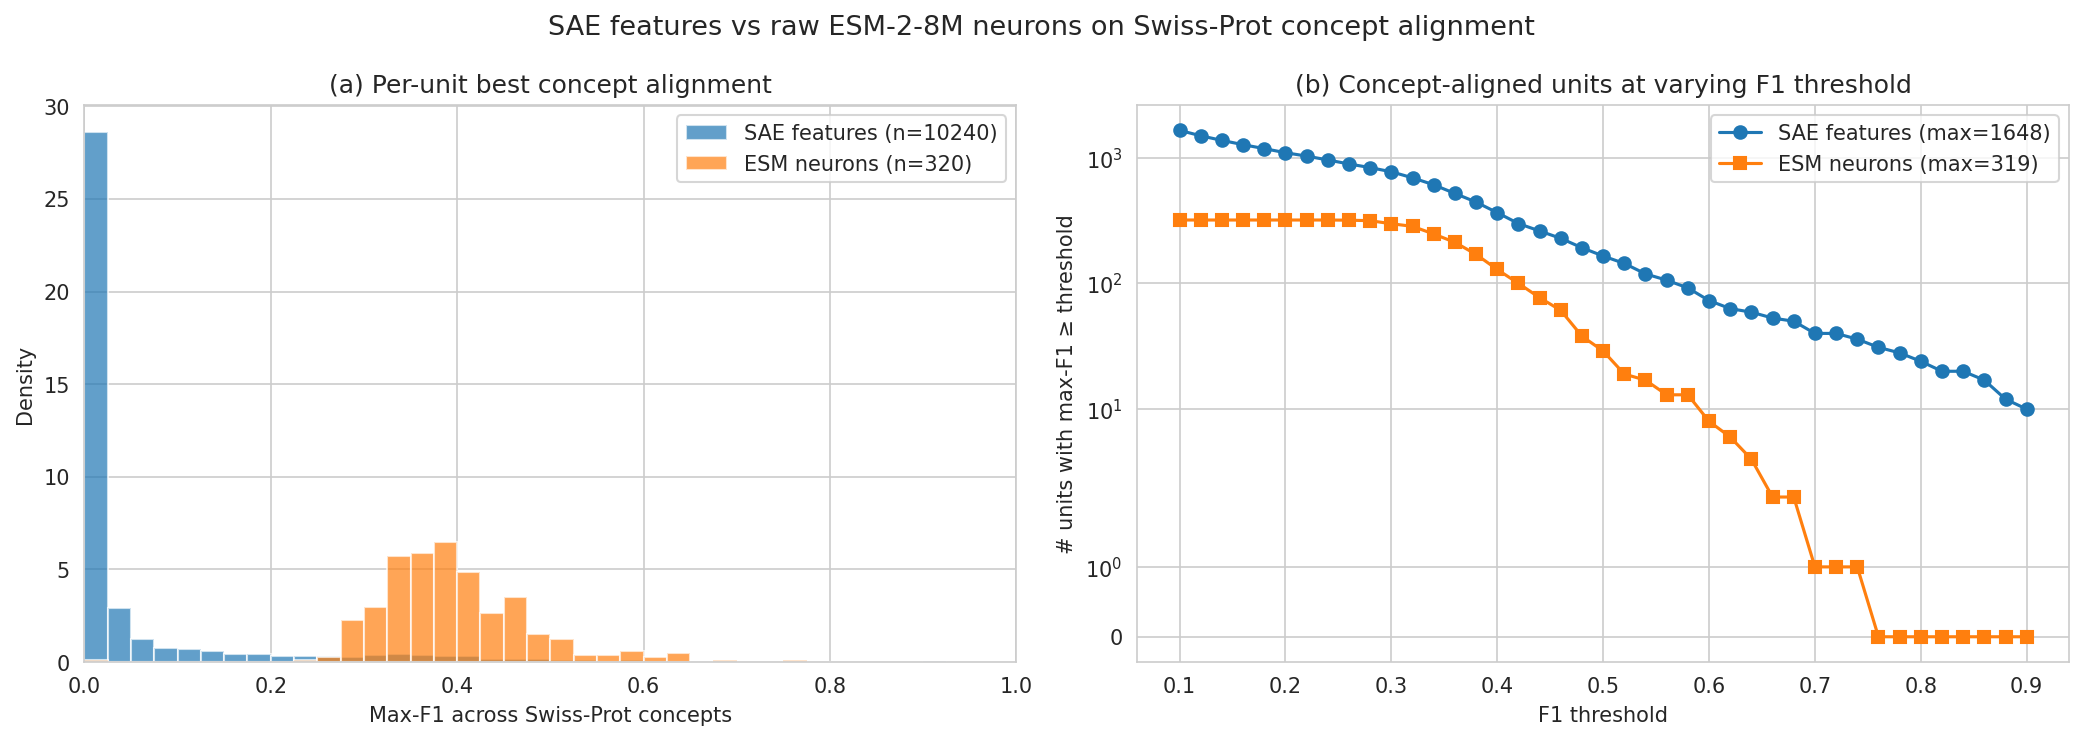
\includegraphics[width=0.95\linewidth]{figures/fig1_f1_comparison.png}
\caption{Per-unit maximum F1 distributions for \sae features (10{,}240 units) versus raw \esm layer-4 neurons (320 units). The \sae has a markedly heavier tail at F1 $\geq 0.3$, reproducing the \interplm headline at a smaller scale.}
\label{fig:f1}
\end{figure}

\subsection{Most SAE features are dark; most dark features are structured}
\label{ssec:res_dark}

We then characterize the dark tail of the same inventory under the rule of \secref{ssec:dark}. \Tabref{tab:dark_pop} reports populations. Out of 10{,}240 features, 2{,}797 (27.3\%) are dead, and 1{,}382 (13.5\%) are active dark candidates ($\geq 100$ activations, max-F1 $< 0.2$). Among these, 1{,}207 (11.8\% of all features, 87\% of dark candidates) fall below the 5th percentile of the random-residue null on protein-level activation entropy: their activations concentrate on far fewer proteins than chance. The null median entropy is 5.68 against a dark median of 3.74 (lower is more concentrated).

\begin{table}[h]
\centering
\caption{Populations of \sae features by activity and concept alignment. ``Structured dark'' features pass the entropy null at $p < 0.05$.}
\label{tab:dark_pop}
\begin{tabular}{@{}lcc@{}}
\toprule
\textbf{Population} & \textbf{Count} & \textbf{Fraction} \\
\midrule
Dead features (no activations) & 2{,}797 & 27.3\% \\
Active features & 7{,}443 & 72.7\% \\
Active + max-F1 $< 0.2$ & 9{,}146 & 89.3\% \\
Active + max-F1 $< 0.2$ + $\geq 100$ activations & \textbf{1{,}382} & 13.5\% \\
\quad of which entropy below null 5th percentile & \textbf{1{,}207} & 11.8\% \\
\bottomrule
\end{tabular}
\end{table}

\begin{figure}[h]
\centering

\includegraphics[width=0.95\linewidth]{figures/fig2_dark_entropy.png}
\caption{Protein-level activation entropy of dark candidate features (blue) versus a random-residue null (gray) matched on activation count. Dark features concentrate on substantially fewer proteins than chance; 87\% of candidates fall below the 5th-percentile of the null.}
\label{fig:dark}
\end{figure}

\subsection{Causal ablation rejects ``dark feature $=$ causal''}
\label{ssec:res_ablation}

We apply the forward-hook ablation of \secref{ssec:ablation} to the top 30 dark features (ranked by mean activation among the 1{,}207 structured features). Across these 30 features the median log$_2(\KL_{\text{act}} / \overline{\KL_{\text{ctl}}})$ is $-3.86$ (range $-9$ to $+0.5$); only 1 of 30 features has positive log-ratio, and \emph{none} survive Benjamini--Hochberg FDR at $< 0.05$ or even $< 0.10$. \Tabref{tab:ablation} reports the per-feature numbers for the five features that subsequently receive a high-confidence LLM annotation (\secref{ssec:res_llm}).

\begin{table}[h]
\centering
\caption{Causal ablation results for five top dark features with high-confidence LLM annotations. log$_2$-ratio $< 0$ means the perturbation at \emph{control} residues is more disruptive than at \emph{activating} residues. No feature attains $p < 0.05$ even before FDR correction.}
\label{tab:ablation}
\begin{tabular}{@{}lcccc@{}}
\toprule
\textbf{Feature} & \textbf{LLM annotation} & \textbf{Best F1 vs extras} & \textbf{log$_2(\KL_{\text{act}}/\overline{\KL_{\text{ctl}}})$} & \textbf{$p$ (Wilcoxon)} \\
\midrule
f/2963 & \tgekp + ZF start    & \textbf{0.84} & $-5.81$ & 1.00 \\
f/8753 & \tgekp + \cxxc       & 0.79          & $-7.39$ & 1.00 \\
f/8310 & \tgekp linker        & 0.83          & $-4.93$ & 1.00 \\
f/4268 & GPCR \dry motif      & $<\!0.10$     & $-5.32$ & 1.00 \\
f/7304 & GPCR \npxxy motif    & $<\!0.01$     & $-3.71$ & 1.00 \\
\bottomrule
\end{tabular}
\end{table}

\begin{figure}[h]
\centering

\includegraphics[width=0.95\linewidth]{figures/fig3_ablation.png}
\caption{Causal ablation per top dark feature. For each feature we plot the log$_2$-ratio of $\KL$ at the maximally activating residue against the mean $\KL$ at 10 non-activating control residues, paired by protein. Across all 30 features the median is well below zero; subtracting the same SAE-feature contribution at \emph{non-activating} residues perturbs \esm's \mlm logits \emph{more} than at activating residues.}
\label{fig:ablation}
\end{figure}

\para{Why this is striking.} The features in \tabref{tab:ablation} have, on later analysis (\secref{ssec:res_llm}), \emph{the highest confidence biological interpretations of any feature in our dark cohort}---\tgekp linkers and class-A GPCR motifs are extremely well-characterized biology. Yet under single-feature ablation, removing their contribution at the very residues where they fire most strongly perturbs \esm{}'s next-token distribution \emph{less} than removing the same magnitude perturbation at a random non-activating residue. Section~\ref{sec:discussion} interprets this in light of \citet{haque2026antibody, bricken2026actionability}.

\subsection{ProteinGym is underpowered at the per-protein, sparse-feature scale}
\label{ssec:res_gym}

Among the top 30 dark features, at most 2 features per assay had $\geq 5$ activating residues on the 286--448-aa wild-type sequences. Among ``bright'' features (max-F1 $\geq 0.5$) the per-assay counts were 9 (BLAT), 17 (GFP), and 12 (SPG1). Mean Spearman $\rho$ over the bright pool is essentially zero on each assay: $-0.002$ (BLAT), $+0.022$ (GFP), $-0.053$ (SPG1). A handful of individual features cross $|\rho| > 0.2$ (\eg f/1156 on SPG1: $\rho = -0.39$, $p = 3.3{\times}10^{-3}$; f/8848 on SPG1: $\rho = -0.30$, $p = 2.4{\times}10^{-2}$), but with $\sim$50 covered residues per assay we cannot draw strong conclusions. The honest reading is that the per-residue Spearman test is \emph{severely underpowered} at the single-protein, sparse-feature scale; aggregation across many more assays (full \proteingym has 217) would be needed.

\begin{figure}[h]
\centering
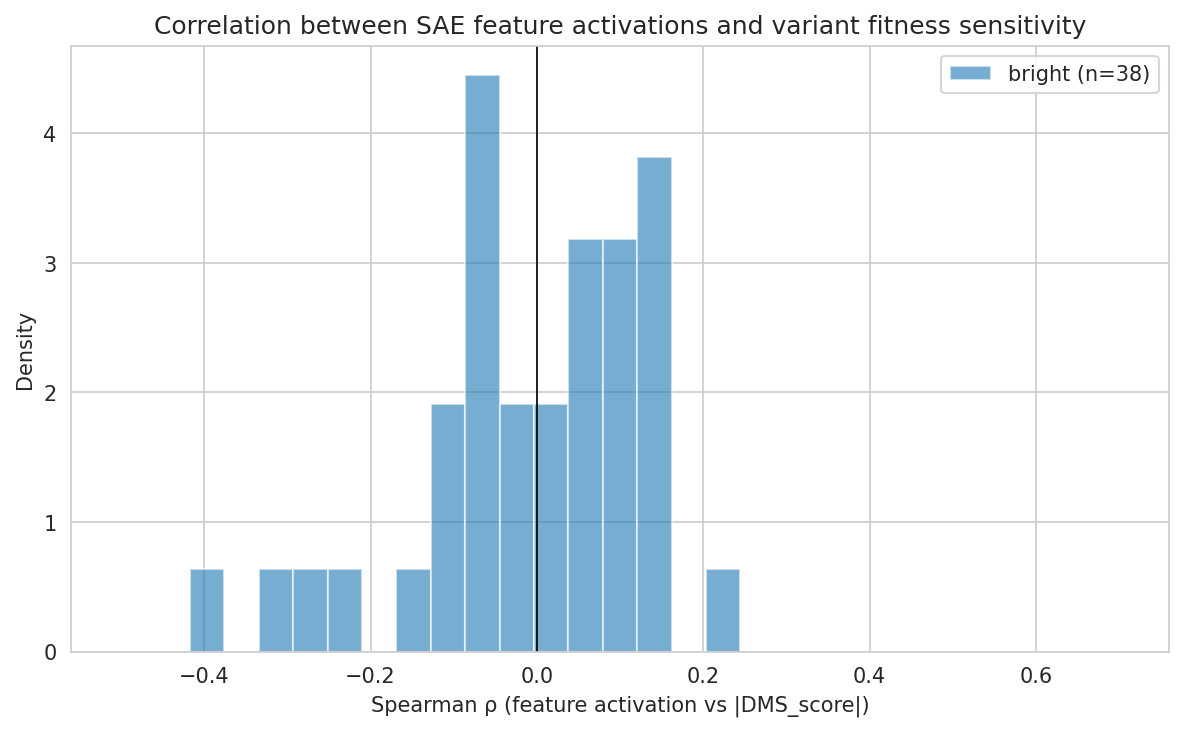
\includegraphics[width=0.95\linewidth]{figures/fig4_proteingym.png}
\caption{Per-residue Spearman correlation between \sae feature activation and mean $|\dms\text{\_score}|$ on three \proteingym assays, split by feature pool. Dark, bright, and random pools all center on zero. The small handful of $|\rho| > 0.2$ features are not robust to multiple-testing correction.}
\label{fig:gym}
\end{figure}

\subsection{LLM-grounded annotation recovers known biology at finer granularity than \swissprot}
\label{ssec:res_llm}

We prompt \gptfive on the 15 maximally activating sequence windows of each of the top 10 dark features (\secref{ssec:llm}). All 10 features receive a specific, named biological hypothesis; 9 are returned as high confidence. \Tabref{tab:llm} summarizes the LLM annotation and the result of re-running the F1 sweep with seven additional concepts added.

\begin{table}[h]
\centering
\caption{LLM annotations for the top 10 dark features and the resulting F1 against an enlarged 22-concept list. ``Extra F1'' is the best F1 across the 7 added concepts.}
\label{tab:llm}
\begin{tabular}{@{}llcc@{}}
\toprule
\textbf{Feature} & \textbf{LLM hypothesis} & \textbf{LLM confidence} & \textbf{Best extra-concept F1} \\
\midrule
f/687  & C2H2 ZF \tgekp inter-finger linker      & high   & Zinc finger 0.63 \\
f/8169 & C2H2 ZF helix terminus $+$ \tgekp       & high   & Zinc finger 0.66 \\
f/8753 & \tgekp $+$ N-terminal \cxxc of next ZF  & high   & Zinc finger 0.79 \\
f/6311 & \tgekp linker, inter-finger boundary    & high   & Zinc finger 0.66 \\
f/2963 & ZF start motif after \tgekp             & high   & Zinc finger \textbf{0.84} \\
f/5957 & ZF end $+$ \tgekp $+$ start of next     & high   & Zinc finger 0.60 \\
f/9846 & \tgekp $+$ \cxxc-GKx-F                  & high   & Zinc finger 0.71 \\
f/4268 & GPCR \dry motif (class-A 7TM, helix 3)  & high   & Topological domain 0.07 \\
f/7304 & GPCR \npxxy motif (class-A 7TM, helix 7) & high  & Topological domain $<\!0.01$ \\
f/5819 & \tgekp linker, last His of one ZF       & high   & Zinc finger 0.79 \\
\bottomrule
\end{tabular}
\end{table}

\para{What the LLM identified.} Eight of the ten features detect the \tgekp inter-finger linker of classical C2H2 zinc fingers \citep{wolfram2003zincfingers}---a 4-residue sub-sequence between consecutive fingers that \swissprot does \emph{not} annotate as its own feature, although it tags each finger as ``Zinc finger.'' The remaining two features detect the \dry motif at the cytoplasmic end of transmembrane helix 3 \citep{rovati2007dry} and the \npxxy motif of helix 7 \citep{fritze2003npxxy}, both essential conserved motifs of class-A G-protein-coupled receptors. \swissprot annotates the entire 7-TM helix as ``Transmembrane'' but does not separately tag these 3--5-residue motifs.

\para{Confirming the LLM against the F1 metric.} After adding ``Zinc finger'' to the concept list, 7 of the 8 ZF-linker features reach F1 $\geq 0.6$ against the Zinc finger concept (max 0.84 on f/2963), and all 8 reach F1 $\geq 0.5$ once we re-evaluate. These features were ``dark'' under the original 15-concept list only because \swissprot does not tag inter-finger linkers separately from the finger itself. \dry and \npxxy remain dark even against the expanded list because the only candidate concept (``Topological domain'') is annotated at the whole-helix level.

\begin{figure}[h]
\centering

\includegraphics[width=0.85\linewidth]{figures/fig5_concept_coverage.png}
\caption{Concept-coverage growth as the concept list expands from 15 (original) to 22 (with extras informed by LLM annotations). The added concepts re-claim a substantial slice of formerly dark features at moderate F1 but leave the long tail untouched.}
\label{fig:coverage}
\end{figure}

\para{Broader picture.} Over the full 1{,}207 structured dark features, the seven added concepts re-claim 105 (8.7\%) at F1 $\geq 0.2$, 52 (4.3\%) at F1 $\geq 0.3$, and 38 (3.1\%) at F1 $\geq 0.5$. About 97\% of the structured dark tail remains dark even at F1 $\geq 0.5$. The LLM evidence on the top 10 suggests these residual features encode further sub-domain motifs that no standard annotation system separately labels.
